\part{Práctica 1}
\section{Práctica 1-1}\label{p11}
\subsection{Actividad 1}\label{p11a1}
\begin{center}
    \parbox{12cm}{\justify\textit{
        Elija 3 bases de datos de la UCI Machine Learning Repository de las que hay en Moodle y transformelas a .arff, indicando en cada una de ellas qué procedimiento ha seguido.
    }}
\end{center}

\subsubsection{Consideraciones generales}\label{ssc:consideraciones-generales}
Para la realización de la tarea he tomado la decisión de editar manualmente los archivos utilizando Visual Studio Code y guardarlos con la extensión \code{.arff}. El paso a csv utilizando excel que se ha sugerido en clase supone varios cambios de formato en los que pueden aparecer diversos problemas como conflictos entre el separador de columnas CSV y el separador de decimales o miles, problemas con el carácter de salto de línea, codificación, etc.

Para conocer los identificadores y tipos de los atributos de cada base de datos he consultado el archivo \code{.names} del directorio de descarga de cada base de datos, que contiene el listado de campos con su nombre, su tipo y sus posibles valores, si procede. He consultado la especificación del formato \code{.arff} en la \href{https://www.cs.waikato.ac.nz/ml/weka/arff.html}{página correspondiente del manual de weka}. Como puede comprobarse en la figura \ref{fig:ejemplo-arff}, un archivo \code{.arff} consta de tres secciones:
\begin{figure}[ht]
    \centering
    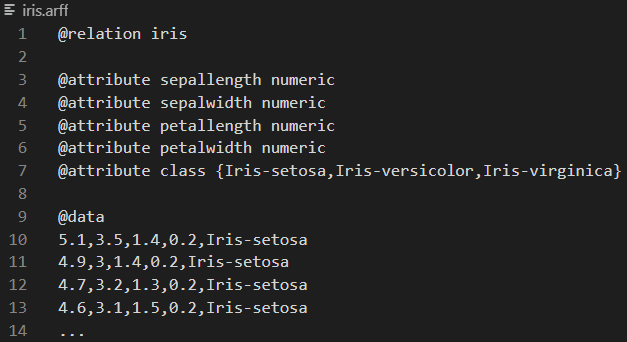
\includegraphics[scale=0.65]{ejemplo-archivo-arff}
    \caption{Ejemplo de archivo \code{.arff}}
    \label{fig:ejemplo-arff}
\end{figure}
\begin{enumerate}
    \item Identificación de la base de datos. Se trata de una línea con el token \code{@relation} seguido por un espacio y el nombre de la base de datos. Por ejemplo: \code{@relation breast-cancer}.
    \item Identificación de los atributos. Tantas líneas como atributos tenga la base de datos, cada una comienza con el token \code{@atribute} seguido del nombre del atributo y el tipo. Los tipos pueden ser:
        \begin{itemize}
            \item Numéricos: \code{@attribute <nombre\string_atributo>\space numeric}
            \item Cadenas de texto: \code{@attribute <nombre\string_atributo> \space string}
            \item Listas de etiquetas: \code{@attribute <nombre\string_atributo> \space\string{valor\string_1, valor\string_2, \dots\string}}
            \item Fechas: \code{@attribute <nombre\string_atributo>\space date [formato\string_de\string_fecha]}. El formato de fecha es opcional, y por defecto acepta ISO-8601 y ``yyyy-MM-dd'T'HH:mm:ss''.
        \end{itemize}
    \item Bloque de datos. Esta sección se inicia con una línea que contiene únicamente palabra clave \code{@data}. A continuación se encontrarán los registros dispuestos en líneas y con sus atributos separados por comas, en el mismo orden en que se han especificado en la cabecera:
    \begin{center}
        \parbox{5.1cm}{\code{@data \\
            v1a1, v1a2, \dots, v1aN \\
            v2a1, v2a2, \dots, v2aN \\
            \dots \\
            vMa1, vMa2, \dots, vMaN
        }}
    \end{center}

\end{enumerate}

\subsubsection{Base de datos \code{breast-cancer}}
Tras aplicar el tratamiento mencionado en el apartado \ref{ssc:consideraciones-generales} al archivo \code{breast-cancer.data} se ha obtenido el fichero \code{.arff} (fig. \ref{fig:breast-cancer-arff}) y una vez cargado en Weka (fig. \ref{fig:breast-cancer-weka}) y se han obtenido las siguientes conclusiones:

\begin{enumerate}
    \item La base de datos tiene 10 atributos, de los cuales el primero es la clase, que toma los valores ``no-recurrence-events'' y ``recurrence-events''. Convendría colocar la clase al final, que es su lugar por defecto.
    \item Los atributos son nominales basados en etiquetas (por ejemplo breast\_quad, menopause\dots) o en rangos numéricos (inv\_nodes, tumor\_size\dots). El atributo deg\_malig se podría poner como numérico ya que parece representar el grado de malignidad en un rango de 1 a 3, por lo que hay una distancia distinta entre los elementos (por ejemplo 1-2 y 1-3).
\end{enumerate}
\begin{figure}[ht]
    \centering
    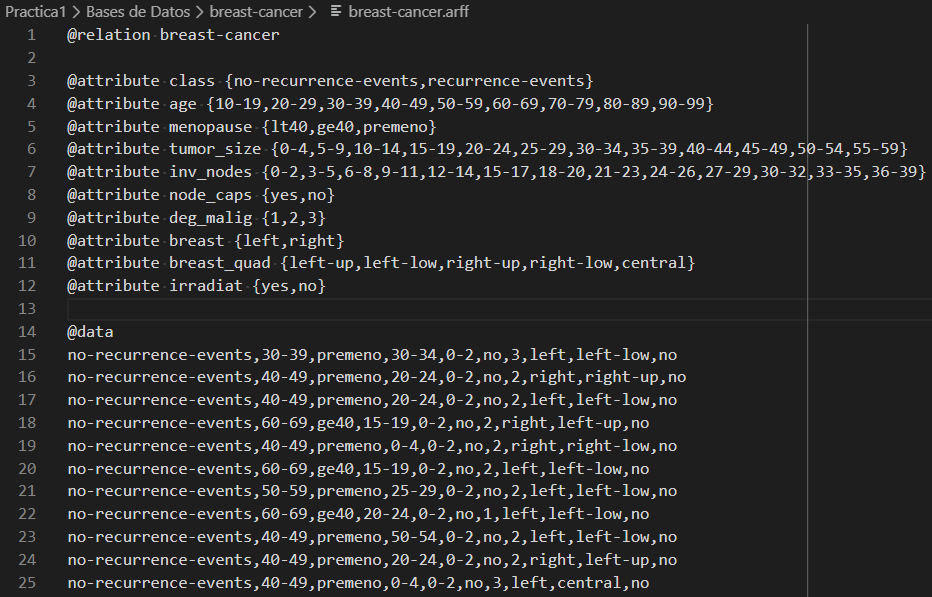
\includegraphics[scale=0.37]{breast-cancer-arff}
    \caption{Captura del archivo \code{breast-cancer.arff}.}
    \label{fig:breast-cancer-arff}
\end{figure}
\begin{figure}[ht]
    \centering
    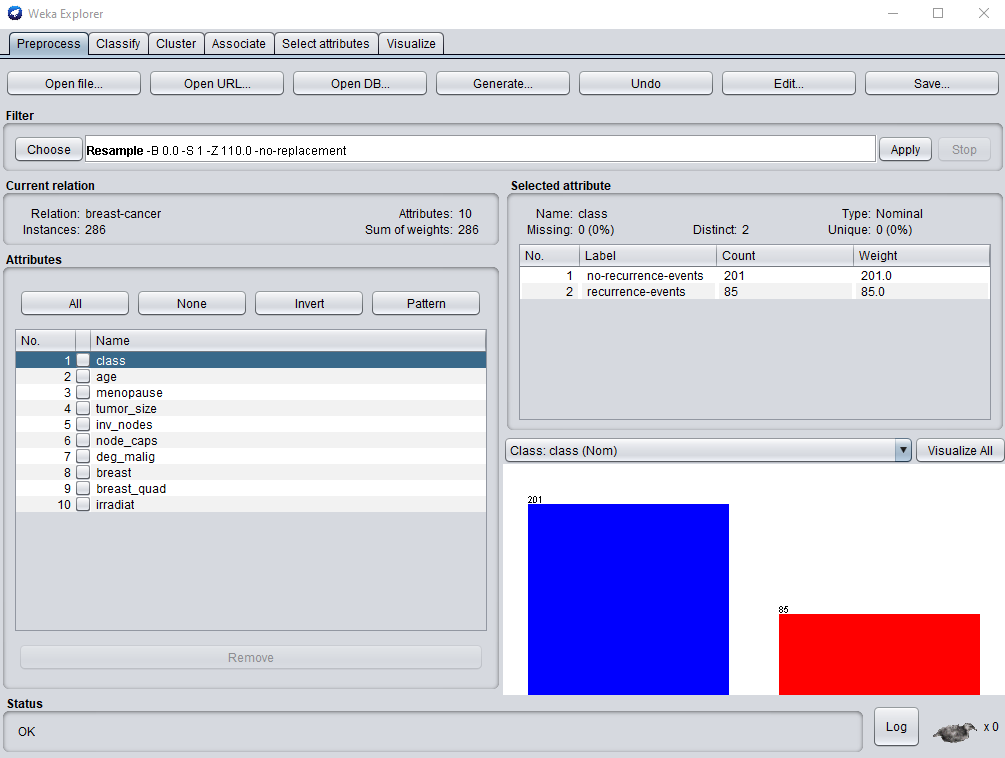
\includegraphics[scale=0.37]{breast-cancer-weka}
    \caption{Archivo \code{breast-cancer.arff} cargado en Weka.}
    \label{fig:breast-cancer-weka}
\end{figure}

\subsubsection{Base de datos \code{dermatology}}
Tras aplicar el tratamiento mencionado en el apartado \ref{ssc:consideraciones-generales} al archivo \code{dermatology.data} se ha obtenido el fichero \code{.arff} (fig. \ref{fig:dermatology-arff}) y una vez cargado en Weka (fig. \ref{fig:dermatology-weka}) y se han obtenido las siguientes conclusiones:

\begin{enumerate}
    \item La base de datos tiene 34 atributos independientes y una clase. En total hay 366 patrones.
    \item La mayoría los atributos son de tipo numérico con valores [0-3]. En la descripción se indica que los valores indican un grado obtenido de un análisis. El caso del atributo family-history es una excepción, ya que es nominal con valores 0 y 1 y representa si alguna de las enfermedades ha sido observada en la familia. Otra excepción es la edad, que siendo numérica, no está restringida al rango anterior.
    \item La clase toma valores de 1 a 6 y cada valor representa un diagnóstico diferente, por lo que es un dato nominal.
\end{enumerate}
\begin{figure}[ht]
    \centering
    \begin{minipage}{0.45\textwidth}
        \centering
        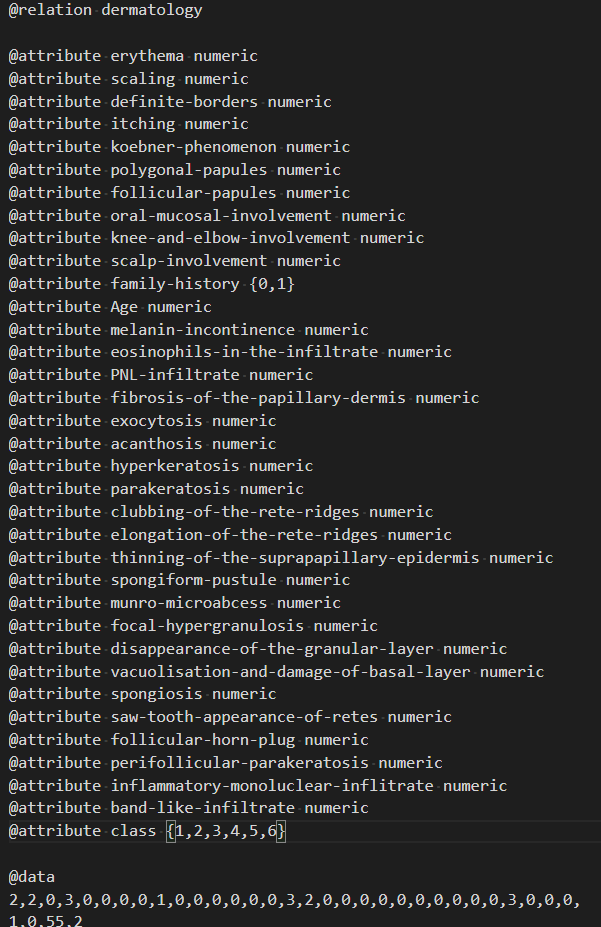
\includegraphics[scale=0.40]{dermatology-arff}
        \caption{Captura de \code{dermatology.arff}.}
        \label{fig:dermatology-arff}
    \end{minipage}\hfill
    \begin{minipage}{0.55\textwidth}
        \centering
        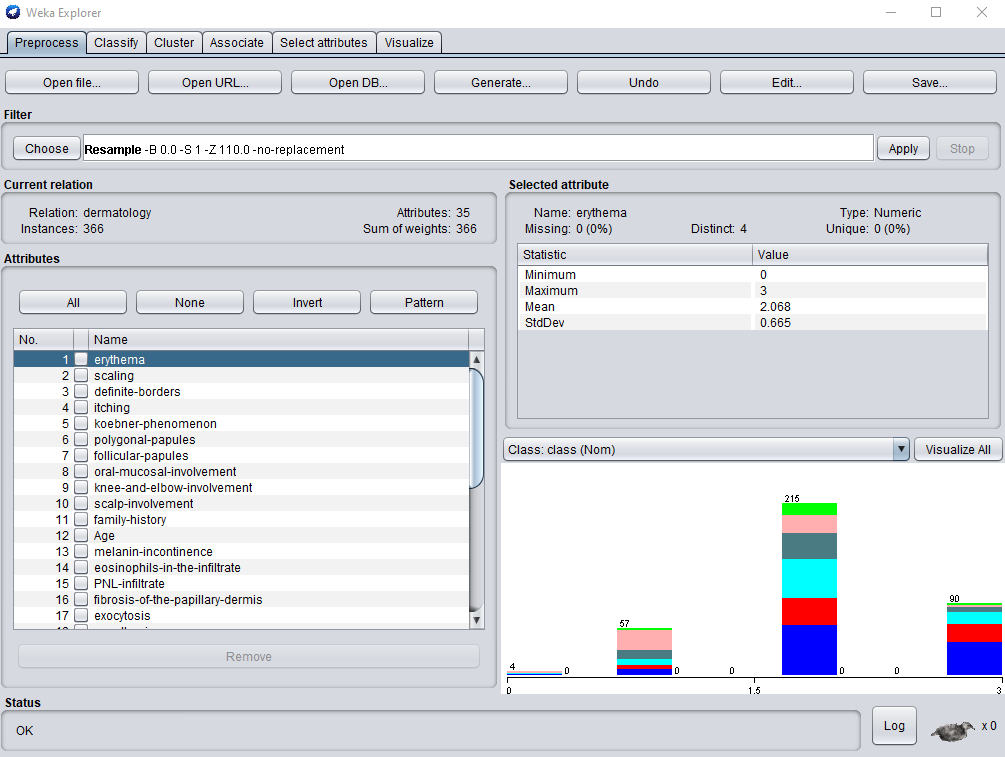
\includegraphics[scale=0.33]{dermatology-weka}
        \caption{Archivo \code{dermatology.arff} cargado en Weka.}
        \label{fig:dermatology-weka}
    \end{minipage}
\end{figure}


\subsubsection{Base de datos \code{wine}}
Tras aplicar el tratamiento mencionado en el apartado \ref{ssc:consideraciones-generales} al archivo \code{wine.data} se ha obtenido el fichero \code{.arff} (fig. \ref{fig:wine-arff}) y una vez cargado en Weka (fig. \ref{fig:wine-weka}) y se han obtenido las siguientes conclusiones:

\begin{enumerate}
\item La base de datos tiene 13 atributos independientes y una clase al principio.
\item Los atributos son numéricos continuos.
\item La clase toma valores 1, 2 o 3 con frecuencias 59, 71 y 48 respectivamente. Es un dato nominal
\end{enumerate}
\begin{figure}[ht]
    \centering
    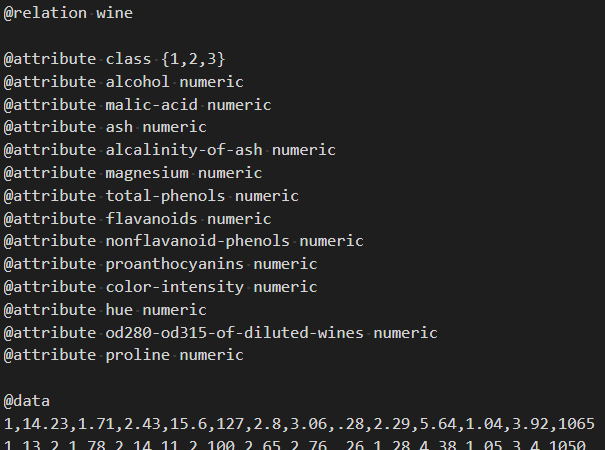
\includegraphics[scale=0.70]{wine-arff}
    \caption{Captura del archivo \code{wine.arff}.}
    \label{fig:wine-arff}
\end{figure}
\begin{figure}[ht]
    \centering
    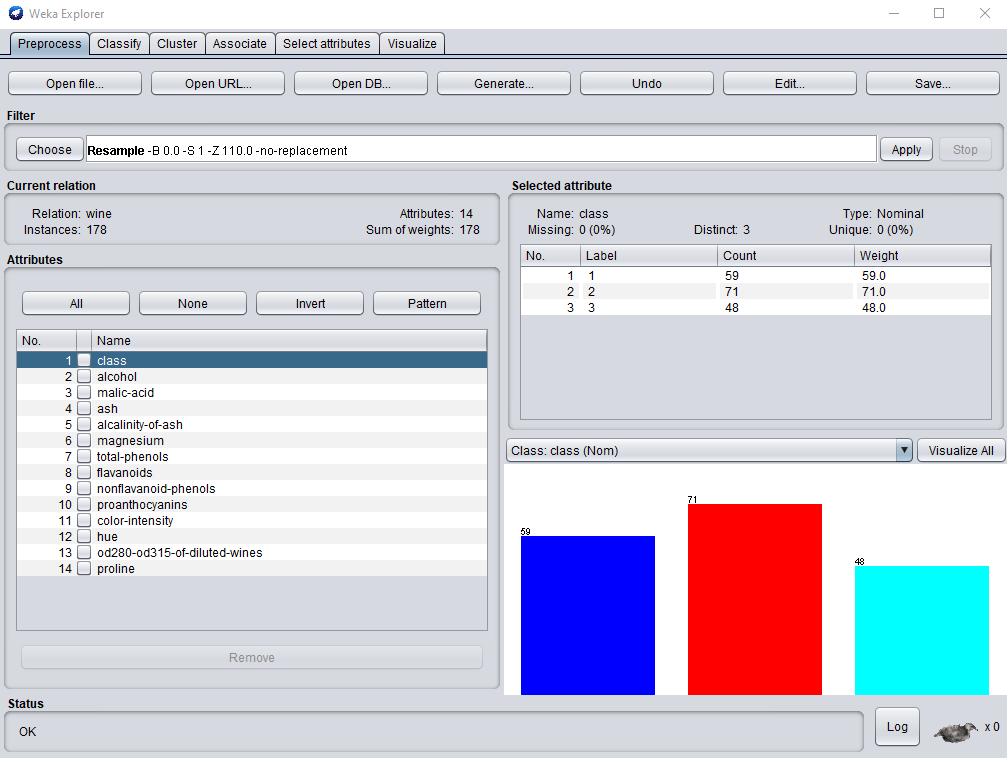
\includegraphics[scale=0.50]{wine-weka}
    \caption{Archivo \code{wine.arff} cargado en Weka.}
    \label{fig:wine-weka}
\end{figure}

\clearpage

\section{Práctica 1-2}\label{p12}
\subsection{Actividad 1}\label{p12a1}
\begin{center}
    \parbox{12cm}{\justify\textit{Elija 3 filtros No Supervisados de los que aparecen listados, expliquelos y describa cómo quedan los datos antes y después al aplicarlos sobre una o varias bases de datos.
    \begin{itemize}
        \item Consulte el UCI Machine Learning Repository para una descripción de la base de datos y la transformación a \code{.arff}
        \item Si no puede aplicar un filtro elegido en ninguna base de datos describa por qué, y constrúyase una base de datos ficticia y pequeña donde si pueda aplicarlo.
        \item Use capturas de pantalla, salidas de Weka y todo lo que considere necesario para sus ejercicios.
        \item La puntuación variará en función de la argumentación y dificultad de los filtros elegidos.
        \begin{enumerate}
            \item filters/unsupervised/attribute/Normalize
            \item filters/unsupervised/attribute/ReplaceMissingValues
            \item filters/unsupervised/attributes/NominalToBinary
            \item filters/unsupervised/intance/RemoveDuplicates
            \item filters/unsupervised/instance/Resample
            \item filters/unsupervised/attribute/Remove
            \item filters/unsupervised/attributes/RemoveUseless
        \end{enumerate}
    \end{itemize}
    }}
\end{center}

\subsubsection{filters/unsupervised/instance/Resample}
\label{ssc:unsupervised-resample}
Según la información que proporciona Weka, este filtro produce un conjunto de datos mediante un remuestreo de la base de datos original. Este remuestreo no supervisado se utiliza para aumentar el número de patrones (\textbf{oversampling}) mediante la creación de duplicados de patrones existentes o para reducirlo (\textbf{undersampling}) mediante la eliminación de patrones aleatorios. La selección de patrones para oversampling se puede hacer con o sin repetición. Si es sin repetición, un patrón duplicado no podrá ser seleccionado de nuevo para su duplicación.

Para ilustrar el comportamiento del filtro observaremos cómo cambian las frecuencias relativas en las clases tras realizar diversos undersamplings y oversamplings. La hipótesis es que las frecuencias relativas no se mantendrán constantes ya que el filtro elimina o duplica patrones al azar. En Weka, se ha cargado la base de datos \code{dermatology.arff}. En la base de datos hay inicialmente 366 patrones repartidos en 6 clases con las frecuencias que se pueden ver en la columna ``Frec. Orig.'' de la tabla \ref{tab:unsupervised-resample-oversample-dist}. Posteriormente, se ha seleccionado el filtro Resample no supervisado: \code{unsupervised/instance/Resample}.

\begin{figure}[ht]
    \centering
    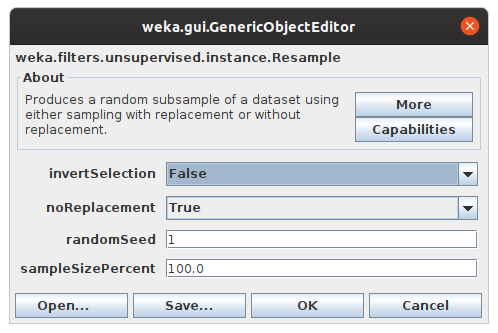
\includegraphics[scale=0.42]{unsupervised-resample}
    \caption{Configuración del filtro \code{unsupervised/Resmaple}.}
    \label{fig:unsupervised-resample}
\end{figure}

El filtro Resample no supervisado cuenta con los siguientes parámetros:

\begin{itemize}
    \item \code{invertSelection False/True}: Invierte la selección (descartados por seleccionados).
    \item \code{noReplacement True/False}: Deshabilita el reemplazo de instancias, esto es, al seleccionar instancias para duplicar, permite o no que la misma instancia sea seleccionada más de una vez. Esto sólo tiene sentido al hacer oversampling (sampleSizePercent>100).
    \item \code{randomSeed (núm 1)}: Semilla para la selección aleatoria.
    \item \code{sampleSizePercent (núm 100)}: Tamaño del conjunto resultante como \% del original.
\end{itemize}

Para este ejercicio se han establecido los siguientes valores de configuración:
\begin {itemize}
    \item \code{randomSeed=50}
    \item \code{noReplacement=True}
    \item \code{invertSelection=False}
    \item \code{sampleSizePercent=\{75, 50, 25\}}.
\end{itemize}

En la tabla \ref{tab:unsupervised-resample-undersample-dist} se muestra la distribución de las clases al utilizar el filtro para realizar \textbf{undersampling} reduciendo el conjunto al 75\%, al 50\% y al 25\%. Cada resample se ha realizado sobre el conjunto original. El proceso ha sido: aplicar el filtro, tomar los datos, deshacer, siguiente.
\begin{table}[ht]
    \centering
    \begin{tabular}{|r|rr|rr|rr|rr|}
        \hline
        \multicolumn{1}{|l|}{Clase} & \multicolumn{2}{r|}{Frec. Orig.} & \multicolumn{2}{r|}{Frec. US75} & \multicolumn{2}{r|}{Frec. US50} & \multicolumn{2}{r|}{Frec. US25} \\ 
        \hline
        1 & 112 & 30,60\% & 87 & 31,75\% & 62 & 33,88\% & 31 & 34,07\% \\
        2 & 61  & 16,67\% & 43 & 15,69\% & 25 & 13,66\% & 13 & 14,29\% \\
        3 & 72  & 19,67\% & 54 & 19,71\% & 37 & 20,22\% & 16 & 17,58\% \\
        4 & 49  & 13,39\% & 37 & 13,50\% & 24 & 13,11\% & 12 & 13,19\% \\
        5 & 52  & 14,21\% & 39 & 14,23\% & 27 & 14,75\% & 16 & 17,58\% \\
        6 & 20  & 5,46\%  & 14 & 5,11\%  & 8  & 4,37\%  & 3  & 3,30\%  \\
        \hline 
        Total\footnote{Porcentajes respecto al tamaño número inicial de patrones} & 366 & 100\% & 274 & 74,86\% & 183 & 50,00\% & 91 & 24,86\% \\
        \hline
    \end{tabular}
    \caption{Frecuencias de clases con diferentes undersamplings}
    \label{tab:unsupervised-resample-undersample-dist}
\end{table}
\begin{figure}[ht]
    \centering
    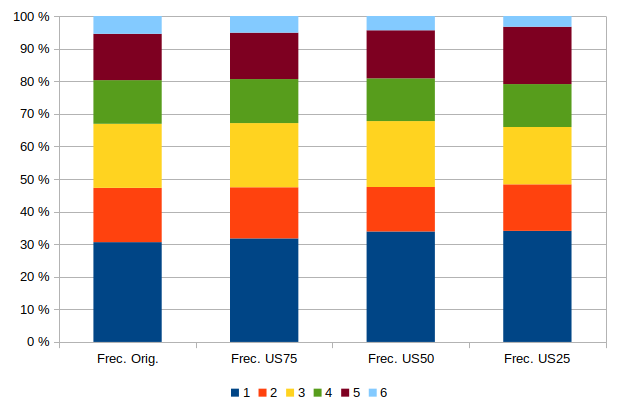
\includegraphics[scale=0.59]{unsupervised-resample-undersample-dist}
    \caption{Frecuencias de clases con diferentes undersamplings}
    \label{fig:unsupervised-resample-undersample-dist}
\end{figure}

Siguiendo la misma dinámica que con el undersampling, se ha realizado un oversampling del conjunto original utilizando el filtro Resample no supervisado, observado que sólo tiene efecto cuando el parámetro \code{noReplacement} se pone a valor \code{False}. En la tabla \ref{tab:unsupervised-resample-oversample-dist} se pueden ver las frecuencias de las diferentes clases al realizar oversamplings al 125\%, 150\%, 175\% y 200\%.

\begin{table}[ht]
    \centering
    \begin{tabular}{|r|rr|rr|rr|rr|rr|}
        \hline
        \multicolumn{1}{|c|}{Clase} & \multicolumn{2}{c|}{Frec. Orig.} & \multicolumn{2}{c|}{Frec. OS125} & \multicolumn{2}{c|}{Frec. OS150} & \multicolumn{2}{c|}{Frec. OS175} & \multicolumn{2}{c|}{Frec. OS200} \\ 
        \hline
        1 & 112 & 30,60\% & 136 & 29,76\% & 168 & 30,60\% & 190 & 29,69\% & 216 & 29,51\% \\
        2 & 61  & 16,67\% & 66  & 14,44\% & 83  & 15,12\% & 100 & 15,63\% & 114 & 15,57\% \\
        3 & 72  & 19,67\% & 89  & 19,47\% & 107 & 19,49\% & 127 & 19,84\% & 149 & 20,36\% \\
        4 & 49  & 13,39\% & 58  & 12,69\% & 68  & 12,39\% & 80  & 12,50\% & 88  & 12,02\% \\
        5 & 52  & 14,21\% & 79  & 17,29\% & 91  & 16,58\% & 104 & 16,25\% & 118 & 16,12\% \\
        6 & 20  & 5,46\%  & 29  & 6,35\%  & 32  & 5,83\%  & 39  & 6,09\%  & 47  & 6,42\%  \\
        \hline
        Total\footnote{Porcentajes respecto al tamaño muestral inicial} & 366 & 100,00 \% & 457 & 124,86 \% & 549          & 150,00 \% & 640 & 174,86 \% & 732 & 200,00 \% \\
        \hline
    \end{tabular}
    \caption{Frecuencias de clases con diferentes oversamplings}
    \label{tab:unsupervised-resample-oversample-dist}
\end{table}
\begin{figure}[ht]
    \centering
    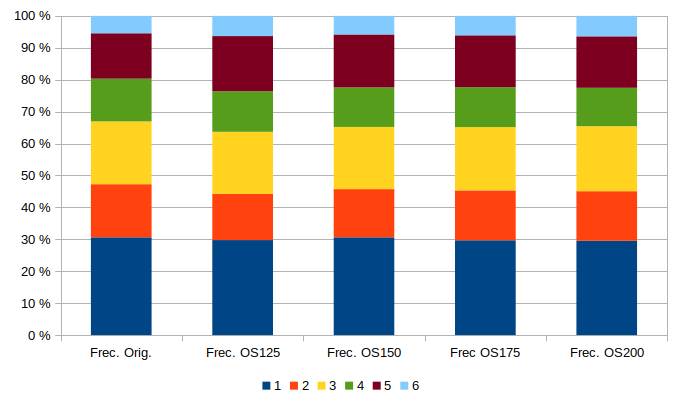
\includegraphics[scale=0.60]{unsupervised-resample-oversample-dist}
    \caption{Frecuencias de clases con diferentes oversamplings}
    \label{fig:unsupervised-resample-oversample-dist}
\end{figure}

Al comparar la frecuencia de cada clase tras las distintas aplicaciones del filtro (fig. \ref{fig:unsupervised-resample-undersample-dist} y \ref{fig:unsupervised-resample-oversample-dist}), se puede observar que varían para los distintos valores de \code{sampleSizePercent}, aunque no demasiado. Dado que se trata de un filtro no supervisado (no tiene en cuenta la clase a la hora de eliminar o crear patrones), este hecho puede deberse a que la base de datos es bastante homogénea en el sentido de que los patrones de cada clase se encuentran distribuidos regularmente a lo largo de la base de datos. En casos de undersampling extremo (ej.: reducción al 4\%) se observa cómo llegan a desaparecer todos los patrones de algunas clases.

En el apartado \ref{ssc:supervised-resample} se probará el filtro supervisado equivalente para comparar las frecuencias obtenidas. Sería lógico suponer que en el filtro supervisado, las frecuencias relativas de las clases variarán menos que en el supervisado según se va reduciendo la muestra.

\subsubsection{filters/unsupervised/attributes/NominalToBinary}

\subsubsection{filters/unsupervised/attributes/RemoveUseless}

%-------------------------------------------------------------------------------
%-------------------------------------------------------------------------------
%-------------------------------------------------------------------------------

\subsection{Actividad 2}\label{p12a2}
\begin{center}
    \parbox{12cm}{\justify\textit{Elija 3 filtros Supervisados de los que aparecen listados, expliquelos y describa cómo quedan los datos antes y después al aplicarlos sobre una o varias bases de datos.
    \begin{itemize}
        \item Consulte el UCI Machine Learning Repository para una descripción de la base de datos y la transformación a \code{.arff}
        \item Si no puede aplicar un filtro elegido en ninguna base de datos describa por qué, y constrúyase una base de datos ficticia y pequeña donde si pueda aplicarlo.
        \item Use capturas de pantalla, salidas de Weka y todo lo que considere necesario para sus ejercicios.
        \item La puntuación variará en función de la argumentación y dificultad de los filtros elegidos.
        \begin{enumerate}
            \item filters/supervised/attribute/Discretize
            \item filters/supervised/attribute/NominalToBinary
            \item filters/supervised/instance/SpreadSubsample
            \item filters/supervised/instance/ClassBalancer
            \item filters/supervised/instance/Resample
        \end{enumerate}
    \end{itemize}
    }}
\end{center}


\subsubsection{filters/supervised/instance/Resample}
\label{ssc:supervised-resample}
El filtro Resample supervisado produce un conjunto de datos mediante un remuestreo de la base de datos original teniendo en cuenta la clase. Este remuestreo supervisado se utiliza para aumentar el número de patrones (\textbf{oversampling}) mediante la creación de duplicados de patrones existentes o para reducirlo (\textbf{undersampling}) mediante la eliminación de patrones manteniendo ciertas proporciones entre los patrones de cada clase. La selección de patrones para oversampling se puede hacer con o sin repetición. Si es sin repetición, un patrón duplicado no podrá ser seleccionado de nuevo para su duplicación. Según la documentación, la clase debe ser de tipo nominal para poder utilizar este filtro. De lo contrario, deberemos utilizar la versión no supervisada \ref{ssc:unsupervised-resample}.

Para ilustrar el comportamiento del filtro observaremos cómo cambian las frecuencias relativas en las clases tras realizar diversos undersamplings y oversamplings en función del valor del parámetro \code{biasToUniformClass}. La hipótesis es que para el valor 0 la distribución de la clase se mantendrá igual mientras que para valor 1 se igualarán. Para valores intermedios del parámetro, mientras más cerca de 1, producirán un resultado más uniforme. En Weka, se ha cargado la base de datos \code{dermatology.arff}. En la base de datos hay inicialmente 366 patrones repartidos en 6 clases con las frecuencias que se pueden ver en la columna ``Frec. Orig.'' de la tabla \ref{tab:unsupervised-resample-oversample-dist}. Posteriormente, se ha seleccionado el filtro Resample supervisado: \code{supervised/instance/Resample}.

\begin{figure}[ht]
    \centering
    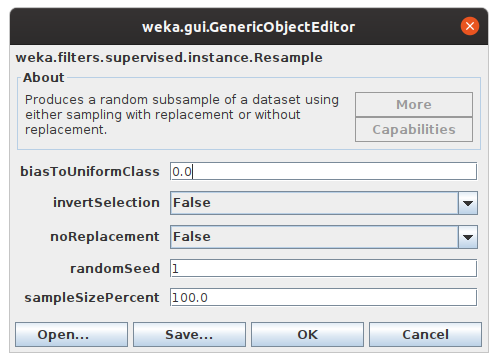
\includegraphics[scale=0.42]{supervised-resample}
    \caption{Configuración del filtro \code{supervised/Resmaple}.}
    \label{fig:supervised-resample}
\end{figure}
El filtro Resample no supervisado cuenta con los siguientes parámetros:

\begin{itemize}
    \item \code{biasToUniformClass (núm [0.0-1.0])}: Establece el tipo de sesgo del remuestreo: para 0 se mantiene distribución original de la clase, para 1, la distribución es uniforme.
    \item \code{invertSelection False/True}: Invierte la selección (descartados por seleccionados).
    \item \code{noReplacement True/False}: Deshabilita el reemplazo de instancias, esto es, al seleccionar instancias para duplicar, permite o no que la misma instancia sea seleccionada más de una vez. Esto sólo tiene sentido al hacer oversampling (sampleSizePercent>100).
    \item \code{randomSeed (núm 1)}: Semilla para la selección aleatoria.
    \item \code{sampleSizePercent (núm 100)}: Tamaño del conjunto resultante como \% del original.
\end{itemize}

Para este ejercicio se han establecido los siguientes valores de configuración:
\begin {itemize}
    \item \code{biasToUniformClass=\{0.0, 1.0\}}
    \item \code{randomSeed=50}
    \item \code{noReplacement=True}
    \item \code{invertSelection=False}
    \item \code{sampleSizePercent=\{33, 66, 150, 200\}}.
\end{itemize}




\begin{table}[ht]
    \centering
    \begin{tabular}{|r|rr|rr|
    >{\columncolor[HTML]{C0C0C0}}r 
    >{\columncolor[HTML]{C0C0C0}}r |rr|rr|}
    \hline
    \multicolumn{1}{|c|}{Clase} &
      \multicolumn{2}{c|}{Frec. US33} &
      \multicolumn{2}{c|}{Frec. US66} &
      \multicolumn{2}{c|}{\cellcolor[HTML]{C0C0C0}Frec. Orig.} &
      \multicolumn{2}{c|}{Frec. OS150} &
      \multicolumn{2}{c|}{Frec. OS200} \\ \hline
      1     & 30  & 25,00\% & 59  & 24,48\% & 112 & 30,60\%  & 142 & 25,87\%  & 196 & 26,78\% \\
      2     & 20  & 16,67\% & 34  & 14,11\% & 61  & 16,67\%  & 92  & 16,76\%  & 122 & 16,67\% \\
      3     & 29  & 24,17\% & 63  & 26,14\% & 72  & 19,67\%  & 120 & 21,86\%  & 153 & 20,90\% \\
      4     & 15  & 12,50\% & 31  & 12,86\% & 49  & 13,39\%  & 78  & 14,21\%  & 97  & 13,25\% \\
      5     & 23  & 19,17\% & 40  & 16,60\% & 52  & 14,21\%  & 87  & 15,85\%  & 122 & 16,67\% \\
      6     & 3   & 2,50\%  & 14  & 5,81\%  & 20  & 5,46\%   & 30  & 5,46\%   & 42  & 5,74\%  \\ \hline
      Total\footnote{Porcentajes respecto al tamaño muestral inicial} & 120 & 32,79\% & 241 & 65,85\% & 366 & 100,00\% & 549 & 150,00\% & 732 & 200,00\% \\ \hline
    \end{tabular}
    \caption{Frecuencias de clases con diferentes resamples y \code{biasToUniformClass=0}}
    \label{tab:supervised-resample-bias0-dist}
\end{table}
\begin{figure}[ht]
    \centering
    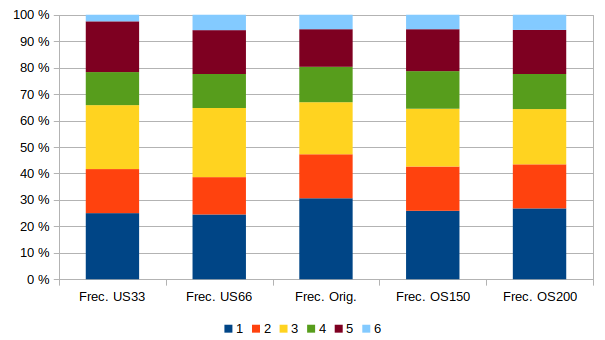
\includegraphics[scale=0.60]{supervised-resample-bias0-dist}
    \caption{Frecuencias de clases al hacer resample con \code{biasToUniformClass=0}}
    \label{fig:supervised-resample-bias0-dist}
\end{figure}






\clearpage




\begin{table}[ht]
    \centering
    \begin{tabular}{|r|rr|rr|
    >{\columncolor[HTML]{C0C0C0}}r 
    >{\columncolor[HTML]{C0C0C0}}r |rr|rr|}
    \hline
    \multicolumn{1}{|c|}{Clase} &
      \multicolumn{2}{c|}{Frec. US33} &
      \multicolumn{2}{c|}{Frec. US66} &
      \multicolumn{2}{c|}{\cellcolor[HTML]{C0C0C0}Frec. Orig.} &
      \multicolumn{2}{c|}{Frec. OS150} &
      \multicolumn{2}{c|}{Frec. OS200} \\ \hline
    1     & 16  & 13,33\% & 43  & 17,84\% & 112 & 30,60\%  & 93  & 16,94\%  & 122 & 16,67\%  \\
    2     & 16  & 13,33\% & 30  & 12,45\% & 61  & 16,67\%  & 88  & 16,03\%  & 120 & 16,39\%  \\
    3     & 26  & 21,67\% & 40  & 16,60\% & 72  & 19,67\%  & 93  & 16,94\%  & 114 & 15,57\%  \\
    4     & 17  & 14,17\% & 36  & 14,94\% & 49  & 13,39\%  & 93  & 16,94\%  & 132 & 18,03\%  \\
    5     & 24  & 20,00\% & 48  & 19,92\% & 52  & 14,21\%  & 97  & 17,67\%  & 123 & 16,80\%  \\
    6     & 21  & 17,50\% & 44  & 18,26\% & 20  & 5,46\%   & 85  & 15,48\%  & 121 & 16,53\%  \\ \hline
    Total\footnote{Porcentajes respecto al tamaño muestral inicial} & 120 & 32,79\% & 241 & 65,85\% & 366 & 100,00\% & 549 & 150,00\% & 732 & 200,00\% \\ \hline
    \end{tabular}
    \caption{Frecuencias de clases con diferentes resamples y \code{biasToUniformClass=1}}
    \label{tab:supervised-resample-bias1-dist}
\end{table}
\begin{figure}[ht]
    \centering
    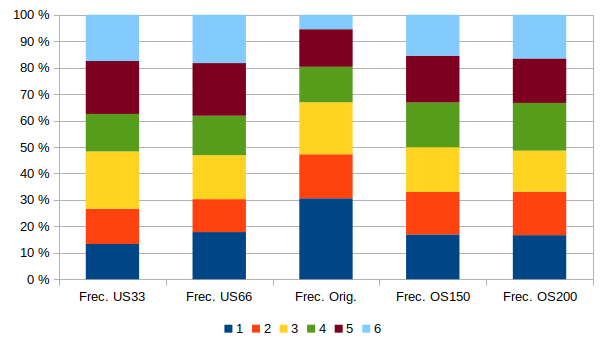
\includegraphics[scale=0.60]{supervised-resample-bias1-dist}
    \caption{Frecuencias de clases al hacer resamples con \code{biasToUniformClass=1}}
    \label{fig:supervised-resample-bias1-dist}
\end{figure}